\documentclass[10pt]{article}
\usepackage[margin=0.83in]{geometry}
\usepackage{amsmath,amssymb,graphicx,booktabs,hyperref,microtype}
\usepackage[T1]{fontenc}
\usepackage{lmodern}
\hypersetup{colorlinks=true,urlcolor=blue,linkcolor=blue}
\title{Exploratory Floquet-Stability Boundaries on the\\ Golden Pancake Three-Body Isola}
\author{Numerical working note --- preliminary, not a discovery claim}
\date{October 12, 2026}
\begin{document}
\maketitle
\vspace{-1em}
\begin{abstract}
We numerically continue a published family of planar, Newtonian, collisionless periodic three-body orbits with masses $(1,\mu,1)$, using a representative orbit at $\mu=0.613$. The family itself and its isola structure were already reported by the Three Body Orbits atlas. We integrate the variational equations along 23 nearby periodic solutions, covering $0.585\leq\mu\leq0.630$, to explore the nontrivial Floquet spectrum. A double-precision computation suggests a bounded interval of spectral stability, approximately $0.59904<\mu<0.61784$, with complex quartets of multipliers outside the unit circle beyond both boundaries. This is an \emph{exploratory numerical result}, not yet a verified novelty claim, a rigorous stability proof, or a submission-ready publication.
\end{abstract}
\section{Background and formulation}
The public Golden Pancake Drama family contains seven representatives on an unequal-mass closed isola, with $\mu$ extending approximately from 0.469 to 0.635 \cite{atlasfamily,atlasabout}. We investigate the continuation passing through the atlas's stable representative, rather than claiming a new orbit family. For $G=1$ the equations are
\begin{equation}
 \ddot{\mathbf q}_i = \sum_{j\ne i}m_j\frac{\mathbf q_j-\mathbf q_i}{\lVert \mathbf q_j-\mathbf q_i\rVert^3},\qquad (m_1,m_2,m_3)=(1,\mu,1).
\end{equation}
We use the collinear initial section $\mathbf q_1=(-1,0)$, $\mathbf q_2=(0,0)$, $\mathbf q_3=(1,0)$, and velocities $\dot{\mathbf q}_1=\dot{\mathbf q}_3=(u,v)$ and $\dot{\mathbf q}_2=-2(u,v)/\mu$. This enforces zero total linear momentum and angular momentum. At fixed $\mu$, a nonlinear least-squares Newton-type corrector solves for $(u,v,T)$ by minimizing the \emph{full twelve-component labeled} return residual $\mathbf X(T)-\mathbf X(0)$. Continuation is performed with small steps in $\mu$.

The state and full $12\times12$ fundamental matrix are integrated with SciPy DOP853 and analytic linearized gravitational forces. Among the twelve Floquet multipliers, eight belong to the approximate neutral symmetry/integral sector; we inspect the other four, selected by separation from unity. For their eigenvalues $\lambda_1,\ldots,\lambda_4$, we monitor
\begin{equation}
 D=2\sum_{i=1}^4\lambda_i^2+8-\left(\sum_{i=1}^4\lambda_i\right)^2.
\end{equation}
For ideal reciprocal pairings $\{\lambda,1/\lambda,\nu,1/\nu\}$, $D=[(\lambda+1/\lambda)-(\nu+1/\nu)]^2$. A sign change from positive to negative indicates a collision of two spectral pairs followed by a complex off-circle quartet (a candidate Hamiltonian--Hopf bifurcation); the multiplier moduli are checked independently.

\section{Numerical observations}
Figure~\ref{fig:stability} shows the leading nontrivial multiplier modulus. On the explored continuation, two crossings are estimated at
\begin{equation}
\mu_{\mathrm L}\approx 0.5990438,\qquad \mu_{\mathrm R}\approx0.6178443.
\end{equation}
The digits are numerical root estimates, \emph{not} uncertainty-certified digits; values rounded to five decimal places are recommended until higher-precision continuation verifies the thresholds. The computed interval width is about 0.01880 in the normalized middle mass. The quartet can move appreciably off the unit circle outside this interval: e.g., $\rho=1.1052$ at $\mu=0.597$ and $\rho=1.0613$ at $\mu=0.618$.
\begin{figure}[ht]
\centering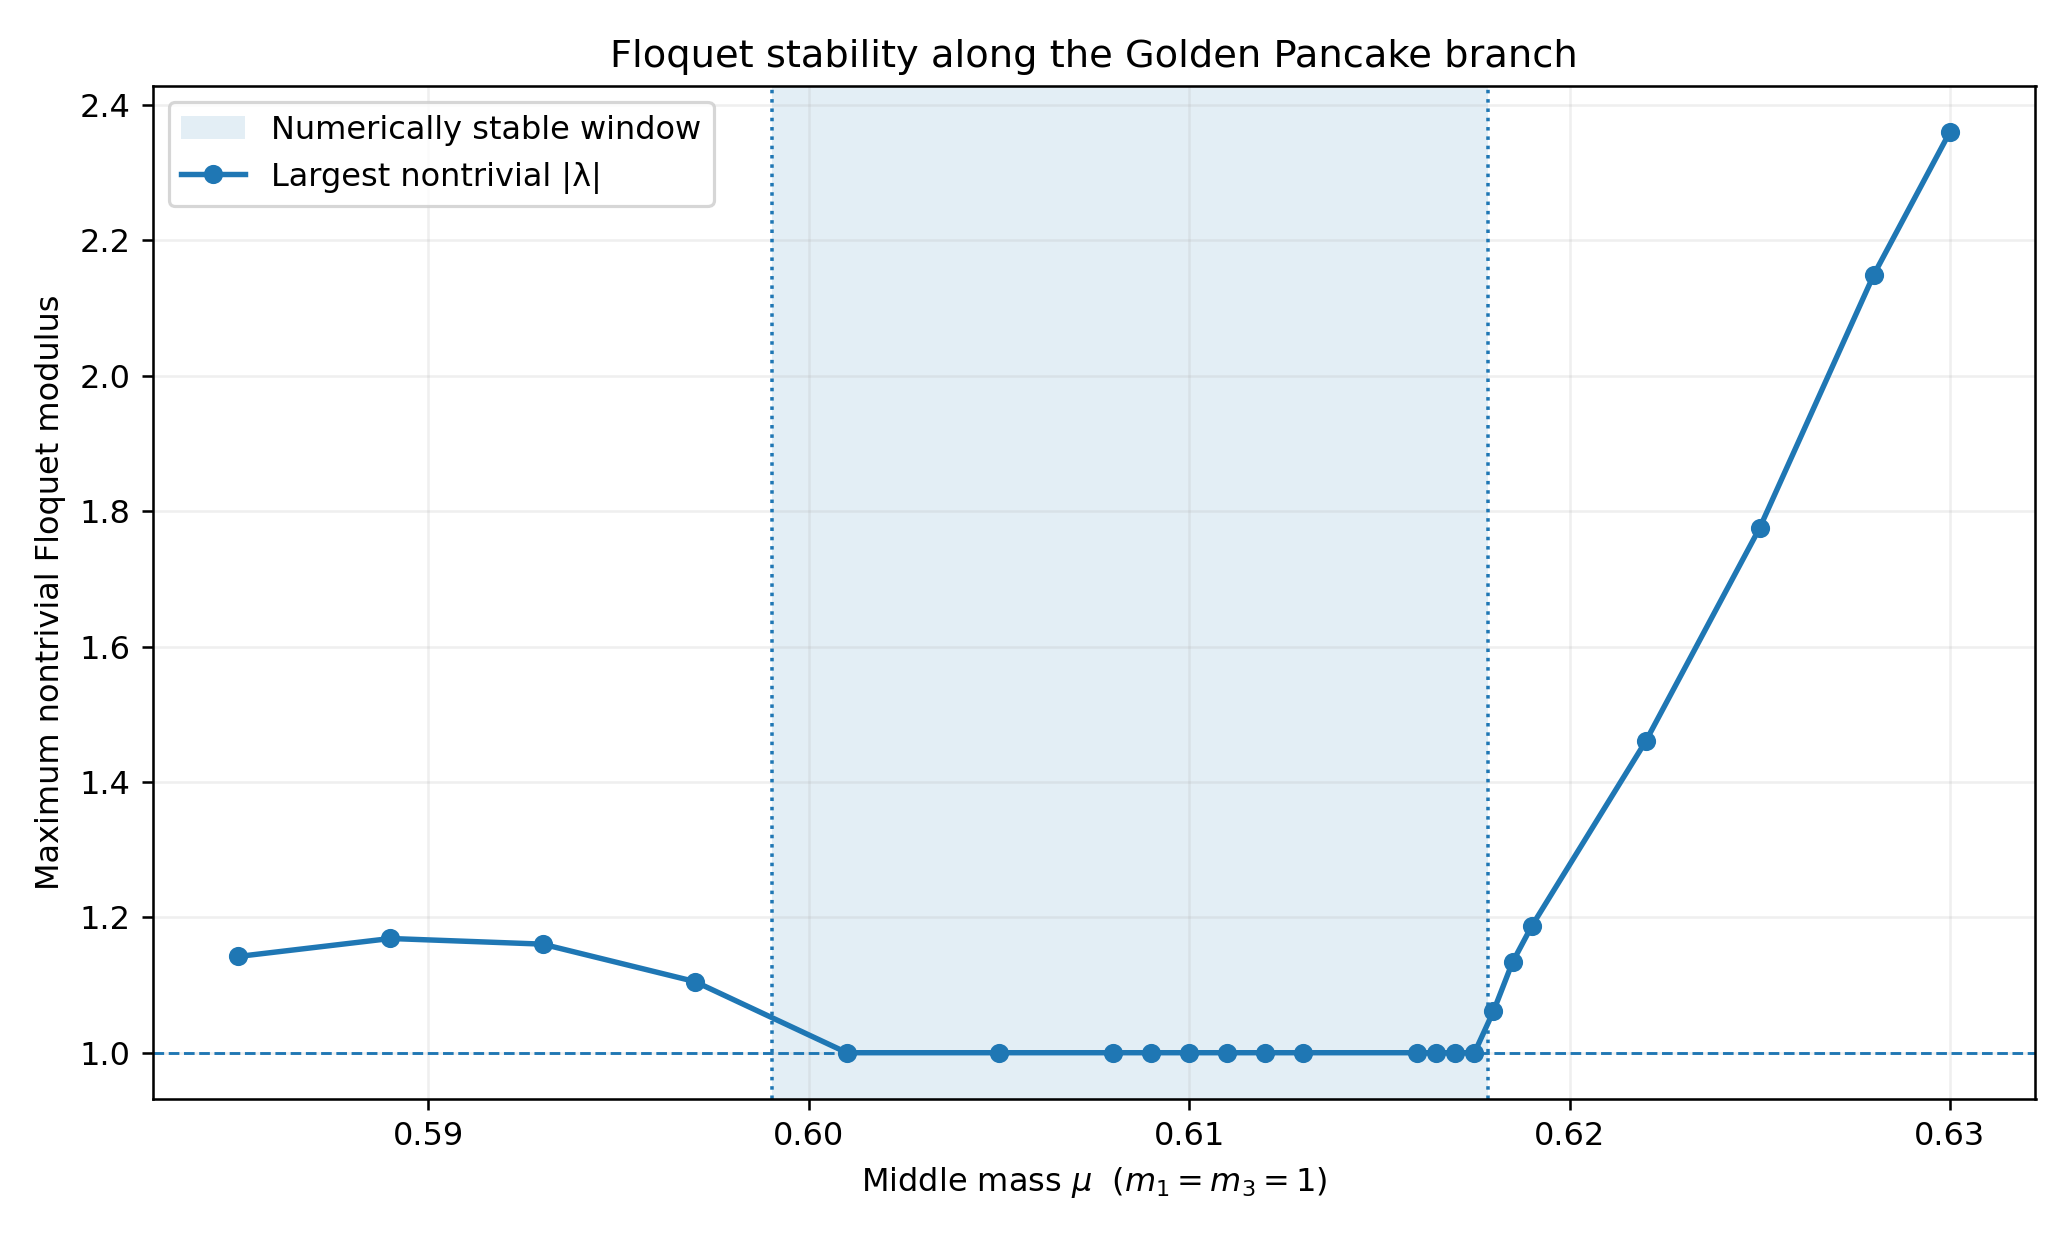
\includegraphics[width=.94\linewidth]{pancake_stability_sweep.png}
\caption{Maximum modulus of the four nontrivial Floquet multipliers for 23 Newton-corrected orbit samples. Shading denotes the inferred stable interval; dotted lines mark the estimated boundaries. Numerical values near the stability threshold remain provisional.}\label{fig:stability}
\end{figure}

\begin{table}[ht]
\centering
\caption{Selected calculations on the same continued branch. $r_{\min}$ is the minimum pairwise separation over one period; $\rho$ is the largest nontrivial Floquet modulus.}
\begin{tabular}{@{}rrrrrl@{}}\toprule
$\mu$ & $T$ & $r_{\min}$ & $D$ & $\rho$ & Spectrum \\ \midrule
0.597 & 8.87705 & 0.01001 & $-0.1309$ & 1.1052 & unstable \\
0.601 & 8.86243 & 0.01075 & $+0.1645$ & 1.0000 & stable candidate \\
0.605 & 8.85129 & 0.01148 & $+0.5702$ & 1.0000 & stable candidate \\
0.613 & 8.84661 & 0.01276 & $+0.9007$ & 1.0000 & stable candidate \\
0.616 & 8.85522 & 0.01310 & $+0.4793$ & 1.0000 & stable candidate \\
0.618 & 8.86617 & 0.01324 & $-0.0482$ & 1.0613 & unstable \\
0.625 & 8.96318 & 0.01261 & $-2.4947$ & 1.7755 & unstable \\
0.630 & 9.14161 & 0.00994 & $-0.7633$ & 2.3604 & unstable \\ \bottomrule
\end{tabular}
\end{table}

\noindent The accompanying file \texttt{pancake\_discriminant\_sweep.png} plots the discriminant across the same 23 masses.



\section{Numerical checks and limitations}
For the 23 sample orbits, the full-state return residuals obtained with the independent reporting integration were about $4.2\times10^{-12}$ to $2.2\times10^{-11}$ in double precision. For five selected masses $\{0.597,0.605,0.613,0.618,0.625\}$, 501 time samples gave maximum absolute energy drift of $4.3$--$6.8\times10^{-12}$ and angular-momentum magnitudes of order $10^{-13}$. Changing the variational-equation integration tolerance between $2\times10^{-12}$ and $9\times10^{-14}$ preserved the discriminant's sign at $\mu=0.5990$, $0.5991$, $0.6178$, and $0.6179$. The 23-point table and those convergence checks are included in the accompanying CSV files, along with runnable source code.

These checks are useful but cannot replace independently converged arbitrary-precision orbit/monodromy calculations. The orbit has pair separations as low as about $0.008$ on this part of the family, making the variational dynamics numerically demanding. The eight neutral multipliers also acquire nonphysical $10^{-4}$-scale deviations from one in double precision due to conditioning; our selected nontrivial quartet is well separated from that neutral cluster. The stability boundaries should be refined with multiprecision shooting, an explicitly symmetry-reduced monodromy matrix, symplectic consistency checks, and an independent Taylor-series or high-order integrator. We did not verify whether these exact stability bounds appear in the atlas authors' full draft PDF, which could not be fetched for text comparison during this study.

\section{Research value and next tests}
The potential contribution is \emph{quantitative stability delimitation along a pre-existing isola}, not the discovery of a new periodic-orbit topology. A serious manuscript should (i) independently verify both critical masses in 50--100-digit arithmetic, (ii) classify the colliding pair's Krein signatures, (iii) resolve the neutral directions using a reduced symplectic return map, (iv) explore asymmetric perturbations $m_1\ne m_3$ to identify a two-parameter stability tongue, and (v) consult and cite the full original research note and authors' existing continuation data. Until these steps are complete, this document is for research planning rather than arXiv submission.

\begin{thebibliography}{9}
\bibitem{atlasfamily} Three Body Orbits, ``Golden pancake drama,'' online family atlas, \url{https://www.threebodyorbits.com/family/golden-pancake-drama} (accessed 2026-10-12).
\bibitem{atlasabout} Three Body Orbits, ``About: how the periodic three-body orbits were computed,'' \url{https://www.threebodyorbits.com/about} (accessed 2026-10-12).
\bibitem{originalnote} Three Body Orbits (2026), ``golden pancake drama: a linearly stable three-body orbit on an unequal-mass isola,'' draft numerical research note, September 9, \url{https://www.threebodyorbits.com/papers/golden-pancake-drama-2026.pdf} (linked by the atlas; full PDF not inspected here).
\bibitem{prior} Vasiljevi\'c, Raoni\'c and Dmitra\v{s}inovi\'c, ``An island of linearly stable non-hierarchical unequal mass periodic three-body orbits,'' \emph{New Astronomy} \textbf{100}, 101969 (2023).
\end{thebibliography}
\end{document}
